\documentclass[12pt]{article}
\usepackage[top=1in, bottom=1in, left=.75in, right=.75in]{geometry}
\usepackage{amsmath, enumerate}
\usepackage{fancyhdr}
\usepackage{graphicx, xcolor, setspace}
\usepackage{txfonts}
\usepackage{multicol,coordsys,pgfplots}
\usepackage[scaled=0.86]{helvet}
\renewcommand{\emph}[1]{\textsf{\textbf{#1}}}
\usepackage{anyfontsize}
% \usepackage{times}
% \usepackage[lf]{MinionPro}
\usepackage{tikz,pgfplots}
%\def\degC{{}^\circ{\rm C}}
\def\ra{\rightarrow}
\usetikzlibrary{calc,arrows.meta}
\usepackage[mathscr]{euscript}
\usepackage{tikz, tkz-euclide}
\usetikzlibrary{calc, through}
\usetikzlibrary{decorations.markings}
\usetikzlibrary{arrows, backgrounds}
\usetikzlibrary{positioning}
\usetikzlibrary{intersections}

\usepackage{adjustbox}
\usepackage{wrapfig}

\pgfplotsset{compat = newest}
\newcommand{\blank}[1]{\rule{#1}{0.75pt}}

\pgfplotsset{my style/.append style={axis x line=middle, axis y line=
middle, xlabel={$x$}, ylabel={$y$}}}

%axis equal

%yticklabels={,,} , xticklabels={,,}

% \setmainfont{Times}
% \def\sansfont{Lucida Grande Bold}
\parindent 0pt
\parskip 4pt
\pagestyle{fancy}
\fancyfoot[C]{\emph{\thepage}}
\fancyfoot[R]{v2}
\fancyhead[L]{\ifnum \value{page} > 1\relax\emph{Math F251X: Midterm 2}\fi}
\fancyhead[R]{\ifnum \value{page} > 1\relax\emph{Fall 2024}\fi}
\headheight 15pt
\renewcommand{\headrulewidth}{0pt}
\renewcommand{\footrulewidth}{0pt}
\let\ds\displaystyle
\def\continued{{\emph {Continued....}}}
\def\continuing{{\emph {Problem \arabic{probcount} continued....}}\par\vskip 4pt}


\newcounter{probcount}
\newcounter{subprobcount}
\newcommand{\thesubproblem}{\emph{\alph{subprobcount}.}}
\def\problem#1{\setcounter{subprobcount}{0}%
\addtocounter{probcount}{1}{\emph{\arabic{probcount}.\hskip 1em(#1)}}\par}
\def\subproblem#1{\par\hangindent=1em\hangafter=0{%
\addtocounter{subprobcount}{1}\thesubproblem\emph{#1}\hskip 1em}}
\def\probskip{\vskip 10pt}
\def\medprobskip{\vskip 2in}
\def\subprobskip{\vskip 45pt}
\def\bigprobskip{\vskip 4in}


\newenvironment{subproblems}{%
\begin{enumerate}%
\setcounter{enumi}{\value{subprobcount}}%
\renewcommand{\theenumi}{\emph{\alph{enumi}}}}%
{\setcounter{subprobcount}{\value{enumi}}\end{enumerate}}


\newcommand{\be}{\begin{enumerate}}
\newcommand{\ee}{\end{enumerate}}


\begin{document}
{\emph{\fontsize{26}{28}\selectfont Fall 2024 \hfill
%{\fontsize{32}{36}\selectfont Calculus 1: Midterm 1}
\hfill Math F251X}}

\begin{center}
{\emph{%\fontsize{26}{28}\selectfont Spring 2024 
%%\hfill
{\fontsize{32}{36}\selectfont Calculus 1: Midterm 2}
%%\hfill Math F251X}
}}
\end{center}

%\vskip 2cm
\strut\vtop{\halign{\emph#\hskip 0.5em\hfil&#\hbox to 2in{\hrulefill}\cr
\emph{\fontsize{18}{22}\selectfont Name:}&\cr
%\noalign{\vskip 10pt}
%\emph{\fontsize{18}{22}\selectfont Student Id:}&\cr
%\noalign{\vskip 10pt}
%\emph{\fontsize{18}{22}\selectfont Calculator Model:}&\cr
}}
\hfill
\vtop{\halign{\emph{\fontsize{18}{22}\selectfont #}\hfil& \emph{\fontsize{18}{22}\selectfont\hskip 0.5ex $\square$ #}\hfil\cr
Section: & 9:15am (James Gossell)\cr
\noalign{\vskip 4pt}
         & 11:45am (Jill Faudree)\cr
\noalign{\vskip 4pt}
         & 11:45am (Leah Berman)\cr
\noalign{\vskip 4pt}
         & async (James Gossell)\cr}}

\vfill
{\fontsize{18}{22}\selectfont\emph{Rules:}}

\begin{itemize}
\item Partial credit may be awarded, but you must show your work.

\item You may have a single handwritten $3'' \times 5''$ notecard, both sides.

\item Calculators are {\bf not} allowed. 

\item Place a box around your  \fbox{FINAL ANSWER} to each question where appropriate.

\item Turn off anything that might go beep during the exam.

\end{itemize}

%If you need extra space, you can use the back sides of the pages.
%Please make it obvious  when you have done so.



Good luck!
\vfill
\def\emptybox{\hbox to 2em{\vrule height 16pt depth 8pt width 0pt\hfil}}
\def\tline{\noalign{\hrule}}
\centerline{\vbox{\offinterlineskip
{
\bf\sf\fontsize{18pt}{22pt}\selectfont
\hrule
\halign{
\vrule#&\strut\quad\hfil#\hfil\quad&\vrule#&\quad\hfil#\hfil\quad
&\vrule#&\quad\hfil#\hfil\quad&\vrule#\cr
height 3pt&\omit&&\omit&&\omit&\cr
&Problem&&Possible&&Score&\cr\tline
height 3pt&\omit&&\omit&&\omit&\cr
&1&&12&&\emptybox&\cr\tline
&2&&10&&\emptybox&\cr\tline
&3&&12&&\emptybox&\cr\tline
&4&&11&&\emptybox&\cr\tline
&5&&12&&\emptybox&\cr\tline
&6&&12&&\emptybox&\cr\tline
&7&&12&&\emptybox&\cr\tline
&8&&9&&\emptybox&\cr\tline
&9&&10&&\emptybox&\cr\tline \tline
&Extra Credit&&5&&\emptybox&\cr\tline
&Total&&100&&\emptybox&\cr
}\hrule}}}

\newpage
%\begin{enumerate}
%%%%

%%%%%%%%%% Limits %%%%%%%%%%%%

\problem{12 points}  Evaluate the following limits. \emph{Show your work}, uncluding appropriate use of limit notation. If you use L'H\^opital's rule, you must indicate where you are using it by writing $\stackrel{H}{=}$ or $\stackrel{L'H}{=}$ or something similar. Use $\infty$ or $-\infty$ where appropriate, and if the limit does not exist, write {\sf DNE} and provide a justification.
\begin{subproblems}
	\item $\displaystyle \lim_{x \rightarrow \infty} \frac{2x-4x^3}{\, x^3-4x^2-6 \,}$
	\vfill
	\item $\displaystyle \lim_{t \rightarrow 3} \frac{e^{t-3}-t+2}{\, t^2-6t+9 \,}$
	\vfill
	\item $\displaystyle \lim_{\theta \rightarrow 0} \frac{2\sin(\theta) - 2}{1-\theta -e^{\cos(\theta)}}$
	\vfill
\end{subproblems}


\newpage

%%%%%%%%%%%%%%%%%%RELATED RATES %%%%%%%%%%%%%%%%%
\problem{10 points} 

A camera at ground level is 100 meters from the landing site of a parachutist who is landing vertically. Let $h$ be the height of the parachutist above the ground and let $\theta$ be the angle of elevation formed between the camera lens and the ground. (See figure.)

\begin{subproblems}
%\begin{multicols}{2}

\item Find an equation relating $h$ and $\theta$.

\hfill 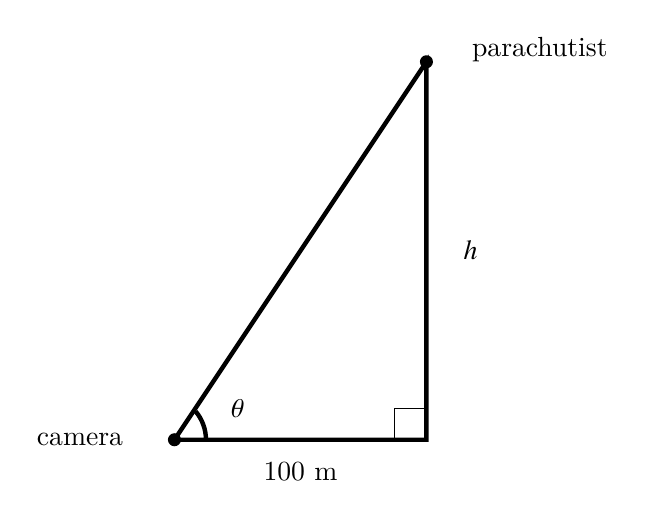
\begin{tikzpicture}[scale=.8]
\draw[ultra thick] (0,0)--(4,0)--(4,6)--(0,0);
\node at (1,0.5){$\theta$};
\draw[ultra thick] (.5,0) arc (0:40:0.7);
\draw (3.5,0)--(3.5,0.5)--(4,0.5);
\node at (2,-.5){ 100 m };
\node at (4.7,3){$h$};
\node at (-1.5,0){camera};
\node[fill,circle,scale=.5] at (4,6){};
\node at (5.8,6.2){parachutist};
\node[fill,circle,scale=.5] at (0,0){};
\end{tikzpicture}

%\vfill

%\end{multicols}

\item Suppose the height of the parachutist decreases at a constant rate of $5$ meters per second. At what rate does the angle $\theta$ decrease when the parachutist is $200$ meters in the air? \emph{Answer the question with a complete sentence, including units.}
	\vfill

\end{subproblems}
\newpage



%\problem{16 points}
%\begin{subproblems}
%\item 
%\end{subproblems}



%\newpage
%%%%%%%%%%%% Optimization

\problem{12 points} 
\def\xx{1}
\def\off{.3}
\def\yy{5} %%%%%% change this for a new problem %%%%%%%%
%Max/min problem
We want to determine the dimensions of the rectangle of maximum area that is inscribed between the parabola $y=\yy-x^2$ and the $x$-axis. Assume the base of the rectangle is on the $x$-axis. (See figure below; the rectangle should be inside the shaded area.) 

	\begin{subproblems}
	
%
%
\begin{minipage}[c]{.5\textwidth}
\begin{tikzpicture}[scale=.8]
  \draw[->] let \n1 = {sqrt(\yy)} in (-\n1 - \off, 0) -- (\n1+\off, 0) node[right] {$x$};
  \draw[->] (0, -\off) -- (0,\yy+\off) node[above] {$y$};
  \draw[<->,domain=-sqrt(\yy)-\off:sqrt(\yy)+\off, smooth, variable=\x, thick] plot ({\x}, {\yy-\x*\x});
 \draw[ultra thick] (-\xx,0)--(\xx,0)--(\xx,\yy-\xx*\xx)--(-\xx,\yy-\xx*\xx)--(-\xx,0);
\draw (\xx, \yy-\xx*\xx) node[right] {$(x, y)$};
\node[circle, fill=black,scale=.5] at (\xx, \yy-\xx*\xx){};
 \begin{scope}[on background layer]
 \filldraw[,domain=-sqrt(\yy):sqrt(\yy), smooth, variable=\x, thick, opacity=.15] plot ({\x}, {\yy-\x*\x});
 \end{scope}
\end{tikzpicture}
\end{minipage}
%
\begin{minipage}{.4\linewidth}
	\item Find an expression for the area $A$ of the rectangle as a function of one variable.

%Note: Your solution must use Calculus to \emph{justify} that your answer is correct.\\
\bigskip
\vspace{1in}
	\item State the appropriate domain of the area function given the context of the problem.
	
		\vspace{1.5cm}

\end{minipage}


%	\vspace{1in}
	\item Use Calculus to determine where the area is maximized. Justify your conclusion with work.
	\vfill
	\item Answer the question: \\
	The dimensions of the rectangle with largest area are \: \blank{6cm}
	\end{subproblems}

%\textbf{answer:} Maximum area is \underline{\hspace{2in}}


%\begin{minipage}{.7\textwidth}
%A manufacturer wants to design a rectangular box with a square base and a fixed volume of 1 $\mathrm{m}^3.$ The material of the base costs \$3 per $\mathrm{m}^2$, the material for the top costs \$2 per $\mathrm{m}^2$, and the material for the sides costs \$5 per $\mathrm{m}^2.$ 
%
%\emph{Determine the dimensions of the box that minimize the cost of construction. }
%
%The formula for the volume of a box is $V=lwh,$ where $l$, $w$, and $h$ represent the length, width, and height of the  box.
%\end{minipage}
%\hfill
%\begin{minipage}{.3\textwidth}
%
%\begin{flushright}
%\begin{tikzpicture}
%\draw[ultra thick] (0,0)--(2,0)--(2,3)--(0,3)--(0,0);
%\draw[ultra thick](0,3)--(1.2,3.6)--(3.2,3.6)--(3.2,0.6)--(2,0)(2,3)--(3.2,3.6);
%\draw[ultra thick, dashed](0,0)--(1.2,0.6)--(3.2,0.6)(1.2,0.6)--(1.2,3.6);
%\node at (1, -0.3){$x$};
%\node at (2.8,0.1){$x$};
%\node at (3.6,2){$y$};
%\end{tikzpicture}
%\end{flushright}
%\end{minipage}
%
%Steps to complete this problem are outlined below.
%%\textcolor{red}{In this version, $x=\sqrt[3]{2}, y=1/2^{2/3}.$}
%
%	\begin{subproblems}
%	\item Find an expression for cost, $C$, as a function of one variable.
%	\vspace{1in}
%	\item State the appropriate domain of the function $C$ given the context of the problem.
%	
%		\vspace{1cm}
%	\item Use Calculus to determine where $C$ is minimized. Justify your conclusion with work.
%	\vfill
%	\item Answer the question: \\
%	The dimensions that minimize cost are $x= \underline{\hspace{1.2in}},\: y=\underline{\hspace{1.2in}}$
%	\end{subproblems}
\newpage
%


%\problem{6 points}
%Suppose the side length of a cube is measured to be 5 cm, with a possible measurement error of $\pm \frac{1}{10}$ cm. 
%\begin{subproblems}
%\item Use linearization or differentials to estimate the possible error in the volume of the cube. 
%
%\vspace{2in}
%
%\item What is the relative error in the volume? %(Show some work.)
%\vspace{1 cm}
%
%\end{subproblems}
%
%\problem{7 points} Find the absolute maximum and absolute minimum for the function %\[\displaystyle{ f(x) = 3x \ln(2x)}\] 
%\[g(x) = (x - 2) (x + 3)^2 = x^3+4 x^2-3 x-18\]
%on the interval $[-4,0].$ Justify how you know that you have found the absolute maximum and minimum. If there is no absolute maximum or minimum write ``none''. %Recall that $e \approx 2.71828$.
%\vfill
%Absolute maximum: $y =$ \hrulefill \ Absoute minimum: $y =$ \hrulefill
%%%%%%%%%%%%%%%%%%%%%%%%
\newpage



%%%%%%%%%%%%%%%%%%%%%%%%%%
\newpage
%%%%%%%%%%%%%%%%%%%%%%%%%%%
%%% Curve Sketching with Algebra %%%%%
\problem{11 points} Consider the function $\ds{g(x) = \frac{x^{2/3}}{x-5}.}$  After  simplification, $\ds{ g'(x) = \frac{-(x+10)}{3x^{1/3}(x-5)^{2}}.}$

\begin{subproblems}
\item What are the critical numbers of $g(x)$?

\vspace{.5in}


\item At what $x$-values does $g(x)$ have local maximum(s)? At what $x$-values does g(x) have local minimum(s)? Clearly show work to \emph{justify} your answers.

\vfill



Local maximum(s): $x = $ \hrulefill \ Local minimum(s): $x = $ \hrulefill

{\it (If none, write ``none''.)}

%{\color{red}
%\item What are the equations of the vertical asymptote(s) of $g(x)$? Justify each answer by writing a limit.
%
%\vfill
%
%Vertical asymptote equation(s): \hrulefill
%
\item Does $g(x)$ have any horizonal asympotes? If it does, write the equations of any horizontal asymptote(s) of $g(x)$, and justify each answer by writing a limit. If it doesn't, explain why $g(x)$ does not have any horizontal asymptotes and write ``none''.


\vfill
Horizontal asymptote equation(s): \hrulefill

(If none, write ``none''.)
%}

\end{subproblems}
\newpage

%%%%%%%%%%%% Curve Sketching with properties
%%%%%%%%%%%%ORIGINAL
%
%\problem{12 points} (ORIGINAL)\emph{Sketch} a graph of a function $f(x)$ that satisfies all of the following properties.
%
%After drawing the graph:
%\begin{itemize}
%\item \emph{Label} on the graph the following things, if they exist, by drawing a point on the graph and labeling: any local maximums by writing  \textsf{LOCAL MAX}, local minimums by writing \textsf{LOCAL MIN}, inflection points by writing \textsf{IP} 
%\item Draw any horizontal and vertical asymptotes with dashed lines and \emph{label} them with their equation.
%\item Mark any important $x$-values and $y$-values on the $x$- and $y$-axes.
%\end{itemize}
%
%\emph{Properties:}
%
%
%\begin{multicols}{2}
%\begin{itemize}
%\item Domain is $(-\infty, \infty)$
%\item $f(0) =0$
%\item $\ds{\lim_{x \to \infty} f(x) = -5}$
%\item $\ds{\lim_{x \to -\infty} f(x) = -\infty}$
%\columnbreak
%\item $f'(x) < 0$ on $(0,4)$
%\item $f'(x) > 0$ on $(\infty,0) \cup (4, \infty)$
%\item $f''(x) < 0$ on $(-\infty, 3) \cup (6,\infty)$
%\item $f''(x) > 0$ on $(3,6)$
%\end{itemize}
%\end{multicols}
%
%
%\begin{tikzpicture}
%\draw[<->] (-8,0) --  (8,0);
%\draw[<->] (0,6) -- (0,-6);
%\end{tikzpicture}
%
%\newpage
%
%%%%%%%%%%% Curve Sketching with properties
%%%%%%%%%%%SUGGESTED

 \problem{12 points} \emph{Sketch} a graph of a function $f(x)$ that satisfies all of the following properties.

After drawing the graph:
\begin{itemize}
\item \emph{Label} on the graph the following things, if they exist, by drawing a point on the graph and labeling: any local maximums by writing  \textsf{LOCAL MAX}, local minimums by writing \textsf{LOCAL MIN}, inflection points by writing \textsf{IP} 
\item Draw any horizontal and vertical asymptotes with dashed lines and \emph{label} them with their equation.
\item Mark any important $x$-values and $y$-values on the $x$- and $y$-axes.
\end{itemize}

\emph{Properties:}


\begin{multicols}{2}
\begin{itemize}
\item Domain is $(-\infty, 1) \cup (1,\infty)$
\item $f(4) = -1$ and $f'(4)=0$
\item $\ds{\lim_{x \to 1^+} f(x) = \infty}$
\columnbreak
\item $f'(x) < 0$ on $(-\infty,1)\cup(1,4)$
\item $f'(x) > 0$ on $(4, \infty)$
\item $f''(x) < 0$ on $(-\infty, 1) \cup (6,\infty)$
\item $f''(x) > 0$ on $(1,6)$
\end{itemize}
\end{multicols}


\begin{tikzpicture}
\draw[<->] (-8,0) --  (8,0);
\draw[<->] (0,6) -- (0,-6);
\end{tikzpicture}

\newpage



%%%%%%%%%%% Curve Sketching given the derivative.
\problem{12 points} The graph shown below is the graph of the \fbox{\emph{derivative $g'(x)$}} of a function $g(x)$. Answer the following questions about the \emph{original} function $g(x)$. %(Do not answer the questions about the picture you are seeing. You need to use that picture to answer the questions about the \emph{original function} $g(x)$.)

%\item 

%\begin{minipage}{.5\linewidth}

\begin{center}
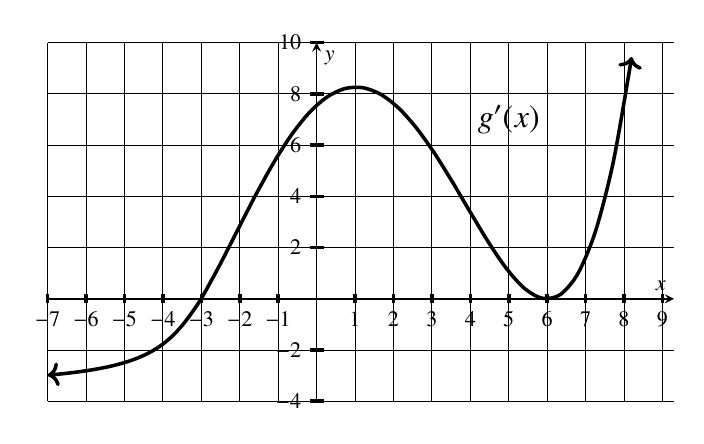
\begin{tikzpicture}[scale = .8]%[yscale=0.4,xscale=1]
\begin{axis}[xscale=1.5, yscale = 1, thick, my style, xtick={-7, ...,9}, ytick={-6,-4,-2,2,4,6,8,10},
xmin=-7, xmax=9.3, ymin=-4, ymax=10, minor y tick num=1,
        minor x tick num=0, mark size=3.0pt, grid=both,   grid style = {black}, tick style = {ultra thick, black}, axis equal image]
  %%%points open
%	\addplot[mark=*,fill=white,only marks] coordinates {(0,-2)(0,3)};
%  \addplot[<-, domain=-1.7:0, smooth, variable=\x, ultra thick] plot ({\x}, {2*(x-1)*(x+1)});
%    \addplot[->, domain=0:4.2, smooth, variable=\x, ultra thick] plot ({\x}, {3/4*(\x-2)*(\x-2)});
%\path (1.5, 2) node {{\Large $g'(x)$}};
%\addplot[ultra thick, smooth, ->] coordinates {(-3,-4)(-4, -2.5)(-4.5,-1)(-4.8, 4)}; 
%\addplot[<->, domain=-4:6, smooth, looseness = 2, line width = .5mm ]coordinates {(-5,4)(-4,0)
%(-3,-1.5)
%(-2,0)
%(-1,4)
%(2,0)
%(3,1)
%(4,2)%
%(6,2.1)};
%\addplot[<-, domain=-6.2:5, smooth, variable=\x, ultra thick] plot ({\x}, {3*1/236*(\x+4)^2*(\x-5)*(\x-7.5)});
\addplot[->, domain=-3:8.2, smooth, variable=\x, ultra thick] plot ({\x}, {3*1/236*((2-\x)+4)^2*((2-\x)-5)*((2-\x)-7.5)});
\addplot[<-, domain=-7:-3, smooth, variable=\x, ultra thick] plot ({\x}, {3*(-0.75)*rad(atan((2-\x)-5))});

%\draw[smooth, ultra thick] (-5,4) to[out = -90, in = 180-60] (-4,0)  parabola bend (-2,-2) (-1,0);
\path (5,7) node {{\Large $g'(x)$}};
\end{axis}
\end{tikzpicture}
\end{center}

\begin{subproblems}

\item Determine the critical numbers of $g(x).$ (Notice that $g(x)$ is \fbox{\emph{not}} shown on the graph!)

	\vspace{1cm}
	

	\item Determine the intervals where $g$ is \emph{increasing} and where $g$ is \emph{decreasing}. If none write ``none''.
	\vfill
		
	Increasing: \hrulefill \hspace{1cm} Decreasing:\hrulefill	
	
	\item Fill in the blanks (if none, write ``none''): 
	
	$g(x)$ has (a) local maximum(s) at $x = $ \blank{1in} and (a) local minimum(s) at $x = \blank{1in} $. 
%\bigskip	
%	\vfill 
	
	\item Find all intervals where $g$ is \emph{concave up} and where $g$ is \emph{concave down}.  (If none write ``none''.)
		\vfill

	Concave up: \hrulefill \hspace{1cm} Concave down:\hrulefill	
	
	
	\item Fill in the blanks: $g(x)$ has (an) inflection point(s) at $x =$ \blank{1in}. (If none, write ``none''.)
	
%	\item \textcolor{red}{ Do we want to ask anything about an asymptote at 0?}

\end{subproblems}

%\end{multicols}

\newpage
%%%%%%%%%%%%%%%%%%%%%%%%%%%%%%%%%%%%

\problem{12 points} The  graph of the function $G(x)$ is below. The function $G(x)$ has domain $[-3,5]$ and the portion of the graph on the interval $[3,5]$ is one quarter of a circle of radius 2 centered at the point $(5,0).$\\
%\textcolor{red}{Easy to version.}
\def\th{.75}
\begin{center}
\begin{tikzpicture}[scale = .7]
%x-axis
\draw[<->,   thick](-4.5,0) -- (6.5,0);
\node at (6.5,-.3){$x$};
%y-axis
\draw[<->,   thick](0,-3.5) -- (0,4.5);
\node at (-.3,4.5){$y$};
%helplines
\draw[help lines, black] (-4,-3) grid (6,4);
\foreach \i in {-4,-3,-2,...,5,6}{
%	\draw (\i,-3)--(\i,4);
	\node at (\i, -0.5){$\i$};
	}
\foreach \i in {-3,-2,-1,1,2,3,4}{
%	\draw (-4,\i)--(6,\i);
	\node at (-0.5,\i){$\i$};
	}
%graph

\filldraw [black,line width = \th mm] (-3,3) circle (2pt);
\draw[line width = \th mm](-3,3) -- (0,3)--(3,0);
\draw[line width = \th mm](3,0) arc (180:270:2);
\filldraw [black, line width = \th mm] (5,-2) circle (2pt);
\end{tikzpicture}
\end{center}

	\begin{subproblems}
%	\item \emph{Approximate} $\ds \int_{-3}^5 G(x) \: dx$ using $R_4,$ a right-endpoint sum using $4$ rectangles. \emph{Draw} the four approximating rectangles on the graph above and lightly shade them in. Your final numerical approximation must be simplified.% as a fraction or exact decimal.
%	\vfill
%	
%	\vfill
%	
%	\vfill
\item Determine $\ds \int_{-2}^3 G(x) \: dx$.

\vfill

	
\item Determine $\ds \int_{-3}^5 G(x) \: dx$.
	
\vfill

\item Determine $\ds \int_{-3}^5 2 G(x) + 3 \: dx$ (Hint: Use part (b) above.)
	\vfill

	\end{subproblems}



\newpage

%%%%%%%%%%%%%%%%%%%%%%%%%
%%%%%%%%%%% Implicit differentiation %%%%%%%%%%%

%\problem{10 points}Below is the graph of the curve $x^4+y^4+2x^2y=21.$
%	\begin{subproblems}
%	\item Write an equation of the line tangent to the curve $x^4+y^4+2x^2y=21$ at the point \textcolor{blue}{$(1,2)$.} %$(2,1)$. 
%	\item  Then \emph{draw} the tangent line on the figure above.
%	\end{subproblems}
%\includegraphics[width = 3in, angle = -90]{mid2-implicit-pic.pdf }
%	
%
%	
%%	\textcolor{red}{Version by using the point $(-2,1)$. -- probably (-1,2)}
%	\vfill
%	
%	Equation of the tangent line at $(1,2)$: \hrulefill 
%	\newpage
%	
%%%%%%%%%%%%%%% Properties of integrals %%%%%%%%%%%%%%

\problem{9 points} 
\begin{minipage}{.5\linewidth} Consider the function 
\[f(x) = \frac{2x}{8-x}.\]
A portion of the graph of this function is shown to the right.

\end{minipage}
\begin{minipage}{.5\linewidth}
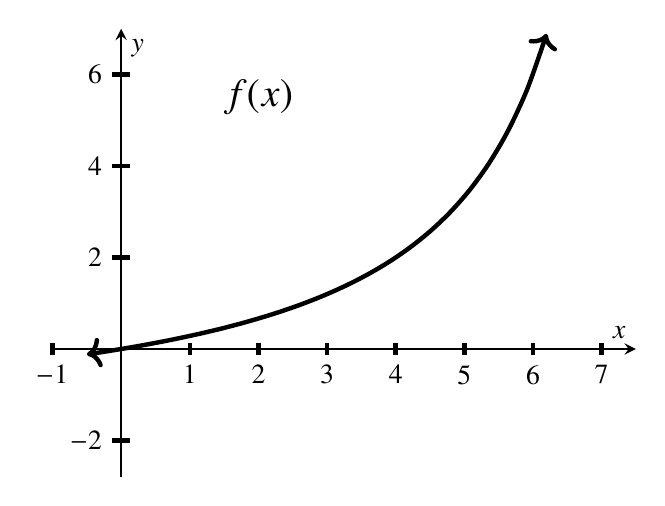
\begin{tikzpicture}[scale = 1]%[yscale=0.4,xscale=1]
\begin{axis}[xscale=1.5, yscale = 1, thick, my style, xtick={-7, ...,12}, ytick={-6,-4,-2,2,4,6,8,10},
xmin=-1, xmax=7.5, ymin=-2.8, ymax=7, minor y tick num=1,
        minor x tick num=0, mark size=3.0pt, grid=none,   grid style = {black}, tick style = {ultra thick, black}, axis equal image]
  %%%points open
%	\addplot[mark=*,fill=white,only marks] coordinates {(0,-2)(0,3)};
%  \addplot[<-, domain=-1.7:0, smooth, variable=\x, ultra thick] plot ({\x}, {2*(x-1)*(x+1)});
%    \addplot[->, domain=0:4.2, smooth, variable=\x, ultra thick] plot ({\x}, {3/4*(\x-2)*(\x-2)});
%\path (1.5, 2) node {{\Large $g'(x)$}};
%\addplot[ultra thick, smooth, ->] coordinates {(-3,-4)(-4, -2.5)(-4.5,-1)(-4.8, 4)}; 
%\addplot[<->, domain=-4:6, smooth, looseness = 2, line width = .5mm ]coordinates {(-5,4)(-4,0)
%(-3,-1.5)
%(-2,0)
%(-1,4)
%(2,0)
%(3,1)
%(4,2)%
%(6,2.1)};
\addplot[<->, domain=-.5:6.2, smooth, variable=\x, ultra thick] plot ({\x}, {2*\x/(8-\x)});
%\addplot[->, domain=5:12, smooth, variable=\x, ultra thick] plot ({\x}, {3*(-0.75)*rad(atan(\x-5))});

%\draw[smooth, ultra thick] (-5,4) to[out = -90, in = 180-60] (-4,0)  parabola bend (-2,-2) (-1,0);
\path (2,5.5) node {{\Large $f(x)$}};
\end{axis}
\end{tikzpicture}


\end{minipage}

\begin{subproblems} 

\item Compute $R_{3}$ on the interval $[0,6]$. That is, approximate $\ds \int_{0}^{6} f(x) \ dx$ using 3 right-hand rectangles. \emph{Draw the rectangles on the graph.}

\vfill

\item List \emph{two distinct strategies} to compute a more accurate approximation of $\ds\int_{0}^{6} f(x)\ dx$.
\vfill
\end{subproblems}

%$\displaystyle \int_0^2 f(x) \:dx = 3$. Use this fact to evaluate the definite integrals below.%	\textcolor{red}{Easy to version.}
%
%	\begin{subproblems}
%	\item $\displaystyle \int_2^0 f(x) \: dx$
%	\vfill
%	\item $\displaystyle \int_0^2 (5f(x)-4) \: dx$
%	\vfill
%	\end{subproblems}
	
%\newpage



%%%%%%%%%% Antiderivatives %%%%%%%%%%%%%%

\problem{10 points}Evaluate the indefinite integrals below. (Give the most generic answer.)

\begin{subproblems} 
%\begin{enumerate}
	\item $\displaystyle \int \left(3x^3 + \cos(x) - e^x + \sqrt{5}\right)\ dx$
	\vfill
	\item $\displaystyle \int \frac{1+x^\frac{1}{3}+x^4}{x}\ dx$
	\vfill
%\end{enumerate}
\end{subproblems}

\newpage


\newpage

%\end{enumerate}
%%%%%%%%%%%%%%%%%%%%%%%%%%%

\fbox{{\bf Extra Credit}} (5 points)
%Compute $\displaystyle \lim_{x\to\infty}\left(1+\frac{1}{x}\right)^{2x}$. \emph{Show your work}.

A population of bacteria can be modeled by the function $\ds P(t) = t^{k/t}$, where $t$ is time, measured in hours, $P$ is the number of bacteria, measured in thousands, and $k$ is a fixed positive constant.

\begin{enumerate}[a.]
\item Compute $\ds \lim_{t\to \infty} P(t)$.
\vfill
\item Interpret this limit by writing a complete sentence, including units, using the context of the model.
\vfill
\end{enumerate}

\end{document}

%%%%ENDDOCUMENT


